% This is a Basic Assignment Paper but with like Code and stuff allowed in it, there is also url, hyperlinks from contents included. 

\documentclass[11pt]{article}

% Preamble

\usepackage[margin=1in]{geometry}
\usepackage{amsfonts, amsmath, amssymb}
\usepackage{fancyhdr, float, graphicx}
\usepackage[utf8]{inputenc} % Required for inputting international characters
\usepackage[T1]{fontenc} % Output font encoding for international characters
\usepackage{fouriernc} % Use the New Century Schoolbook font
\usepackage[nottoc, notlot, notlof]{tocbibind}
\usepackage{listings}
\usepackage{xcolor}
\usepackage{blindtext}
\usepackage{hyperref}
\hypersetup{
    colorlinks=true,
    linkcolor=black,
    filecolor=magenta,      
    urlcolor=cyan,
    pdfpagemode=FullScreen,
    }

\definecolor{codegreen}{rgb}{0,0.6,0}
\definecolor{codegray}{rgb}{0.5,0.5,0.5}
\definecolor{codepurple}{rgb}{0.58,0,0.82}
\definecolor{backcolour}{rgb}{0.95,0.95,0.92}

\lstdefinestyle{mystyle}{
    backgroundcolor=\color{backcolour},   
    commentstyle=\color{codegreen},
    keywordstyle=\color{magenta},
    numberstyle=\tiny\color{codegray},
    stringstyle=\color{codepurple},
    basicstyle=\ttfamily\footnotesize,
    breakatwhitespace=false,         
    breaklines=true,                 
    captionpos=b,                    
    keepspaces=true,                 
    numbers=left,                    
    numbersep=5pt,                  
    showspaces=false,                
    showstringspaces=false,
    showtabs=false,                  
    tabsize=2
}

\lstset{style=mystyle}

% Header and Footer
\pagestyle{fancy}
\fancyhead{}
\fancyfoot{}
\fancyhead[L]{\textit{\Large{Information and Cycbersecurity - 2nd Year B. Tech}}}
%\fancyhead[R]{\textit{something}}
\fancyfoot[C]{\thepage}
\renewcommand{\footrulewidth}{1pt}



% Other Doc Editing
% \parindent 0ex
%\renewcommand{\baselinestretch}{1.5}

\begin{document}

\begin{titlepage}
    \centering

    %---------------------------NAMES-------------------------------

    \huge\textsc{
        MIT World Peace University
    }\\

    \vspace{0.75\baselineskip} % space after Uni Name

    \LARGE{
        Information and Cybersecurity\\
        Second Year B. Tech, Semester 1
    }

    \vfill % space after Sub Name

    %--------------------------TITLE-------------------------------

    \rule{\textwidth}{1.6pt}\vspace*{-\baselineskip}\vspace*{2pt}
    \rule{\textwidth}{0.6pt}
    \vspace{0.75\baselineskip} % Whitespace above the title



    \huge{\textsc{
            Implementation of Diffie - Hellman Key Exchange
        }} \\



    \vspace{0.5\baselineskip} % Whitespace below the title
    \rule{\textwidth}{0.6pt}\vspace*{-\baselineskip}\vspace*{2.8pt}
    \rule{\textwidth}{1.6pt}

    \vspace{1\baselineskip} % Whitespace after the title block

    %--------------------------SUBTITLE --------------------------	

    \LARGE\textsc{
        Lab Assignment 6
    } % Subtitle or further description
    \vfill

    %--------------------------AUTHOR-------------------------------

    Prepared By
    \vspace{0.5\baselineskip} % Whitespace before the editors

    \Large{
        Krishnaraj Thadesar \\
        Cyber Security and Forensics\\
        Batch A1, PA 20
    }


    \vspace{0.5\baselineskip} % Whitespace below the editor list
    \today

\end{titlepage}


\tableofcontents
\thispagestyle{empty}
\clearpage

\setcounter{page}{1}

\section{Aim}
Write a program using JAVA or Python or C++ to implement Diffie-Hellman Key Exchange Algorithm

\section{Objectives}
To learn how to distribute the key.

\section{Theory}

\subsection{What is the Diffie-Hellman Key Exchange Algorithm?}

Diffie-Hellman key exchange is a cryptographic protocol that allows two parties to establish a shared secret key over an insecure communication channel without any prior knowledge of each other. The protocol is based on the discrete logarithm problem and modular arithmetic, and it is widely used in secure communication systems such as SSL/TLS, VPNs, and SSH.

\subsection{Working of the Algorithm}

Here's how the Diffie-Hellman key exchange works, using a simple example:

\begin{enumerate}
    \item Alice and Bob agree on a large prime number p and a primitive root of p, g. These values are public and can be shared over an insecure channel.
    \item Alice chooses a random secret number a and computes $ A = g^a $ mod p. She sends A to Bob over the insecure channel.
    \item Bob chooses a random secret number b and computes $B = g^b$ mod p. He sends B to Alice over the insecure channel.
    \item Alice computes the shared secret key as $K = B^a$ mod p.
    \item Bob computes the shared secret key as $K = A^b$ mod p.
\end{enumerate}

\begin{figure}[H]
    \centering
    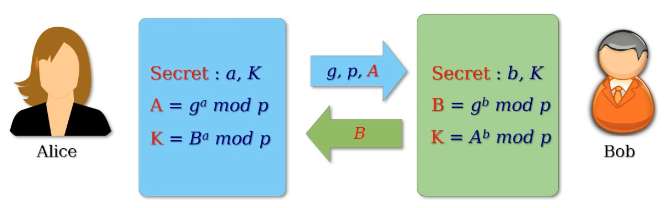
\includegraphics[width=.85\textwidth]{dh.png}
    \caption{Diffie Hellman Protocol}
\end{figure}

Both Alice and Bob end up with the same shared secret key K, which can be used for further encryption and decryption of messages.

\subsection{Example}
Alice and Bob agree on a large prime number $p=11$ and a primitive root of $p$, $g=2$. These values are public and can be shared over an insecure channel.

\begin{enumerate}
    \item Alice chooses a random secret number $a=7$ and computes $A = g^a \bmod p = 2^7 \bmod 11 = 7$. She sends $A=7$ to Bob over the insecure channel.
    \item Bob chooses a random secret number $b=5$ and computes $B = g^b \bmod p = 2^5 \bmod 11 = 10$. He sends $B=10$ to Alice over the insecure channel.
    \item Alice receives $B=10$ from Bob and computes the shared secret key as $K = B^a \bmod p = 10^7 \bmod 11 = 7$.
    \item Bob receives $A=7$ from Alice and computes the shared secret key as $K = A^b \bmod p = 7^5 \bmod 11 = 10$.
\end{enumerate}

Now Alice and Bob both have the same shared secret key $K=7=10$, which they can use to encrypt and decrypt their messages using a symmetric encryption algorithm such as AES.




\section{Platform}
\textbf{\textbf{Operating System}}: Arch Linux x86-64 \\
\textbf{\textbf{IDEs or Text Editors Used}}: Visual Studio Code\\
\textbf{\textbf{Compilers or Interpreters} }: Python 3.10.1\\

\section{Input and Output}

\begin{verbatim}
p:  239
g:  7
Shared secret key from A 95
Shared secret key from B 95
\end{verbatim}


\section{Code}
\lstinputlisting[language=Python, caption="SHA Integrity Check"]{../Programs/Assignment_6/diffie_hellman.py}

\section{Conclusion}
Thus, we have successfully implemented the Diffie-Hellman Key Exchange Algorithm. We learnt about the working of the algorithm and how it is used to distribute any key between 2 parties.
\clearpage

\section{FAQ}

\begin{enumerate}
    \item \textbf{What are other key exchange protocols, other than DH algorithm?}

          \begin{enumerate}
              \item \textbf{RSA Key Exchange}: This protocol uses the RSA algorithm to exchange keys securely between two parties.
              \item \textbf{Elliptic Curve Diffie-Hellman (ECDH)}: This is a variant of the DH algorithm that uses elliptic curve cryptography to provide stronger security and more efficient key exchange.
              \item \textbf{Kerberos}: This is a network authentication protocol that uses a trusted third party (a Key Distribution Center or KDC) to distribute secret keys between two parties.
              \item \textbf{Secure Remote Password (SRP)}: This is a password-based key exchange protocol that allows two parties to establish a shared secret key without revealing their passwords to each other or to an eavesdropper.
              \item \textbf{Signal Protocol}: This is a modern and widely used protocol for secure messaging that uses a combination of the Double Ratchet Algorithm and the DH algorithm to perform key exchange.
              \item \textbf{Station-to-Station (STS)}: This is a protocol that combines elements of the DH and RSA key exchange protocols to provide stronger security and more efficient key exchange.
          \end{enumerate}

    \item \textbf{Explain the different types of keys.}\\

          In cryptography, keys refer to the secret values used for encryption and decryption of messages.

          \begin{enumerate}

              \item \textbf{Symmetric Keys}: Also known as shared keys, these are secret keys that are used for both encryption and decryption of messages. The same key is used by both the sender and the receiver. Examples of symmetric key algorithms include AES, DES, and Blowfish.

              \item \textbf{Public Keys}: Also known as asymmetric keys, these are key pairs consisting of a public key and a private key. The public key is widely distributed and is used for encryption, while the private key is kept secret and is used for decryption. Examples of public key algorithms include RSA, Diffie-Hellman, and elliptic curve cryptography.

              \item \textbf{Session Keys}: These are temporary symmetric keys that are generated for a single session of communication between two parties. They are used to encrypt and decrypt messages exchanged during the session and are discarded once the session is over. Session keys are often used to provide forward secrecy, which means that compromising one session's key does not compromise the security of past or future sessions.

              \item \textbf{Key Exchange Keys}: These are public keys used specifically for exchanging symmetric keys between two parties. Key exchange algorithms like Diffie-Hellman and Elliptic Curve Diffie-Hellman are used to establish a shared secret key between two parties without actually transmitting the key over the communication channel.

          \end{enumerate}

    \item \textbf{Explain different key management issues.}\\

          Key management is the process of securely generating, storing, distributing, and revoking cryptographic keys. Here are some of the most common key management issues in cryptography:

          \begin{enumerate}
              \item \textbf{Key Generation}: The process of generating strong cryptographic keys is essential to ensuring the security of cryptographic systems. However, generating keys that are both random and unpredictable can be difficult. Key generation must be done securely, and the keys must be protected from disclosure or compromise.

              \item \textbf{Key Storage}: Cryptographic keys must be securely stored to prevent unauthorized access or disclosure. The storage of keys is often the weakest link in key management. Keys must be stored in a secure environment, and access to the keys must be tightly controlled.

              \item \textbf{Key Distribution}: Cryptographic keys must be securely distributed to all parties involved in the communication. Key distribution can be challenging, especially when there are multiple parties involved. Key exchange protocols like Diffie-Hellman and RSA can be used to securely exchange keys between parties.

              \item \textbf{Key Revocation}: Keys must be revoked when they are no longer needed or when they have been compromised. Revocation is necessary to prevent unauthorized access to data that was encrypted using the compromised key. Revocation can be challenging, especially in large systems where there are many keys in use.

              \item \textbf{Key Expiration}: Cryptographic keys have a limited lifespan, and must be periodically updated or replaced to maintain their security. Key expiration policies must be carefully designed to balance security and usability.

          \end{enumerate}

\end{enumerate}

\end{document}